\documentclass[border=1pt]{standalone}
\usepackage{tikz}
\usetikzlibrary{calc}

\begin{document}
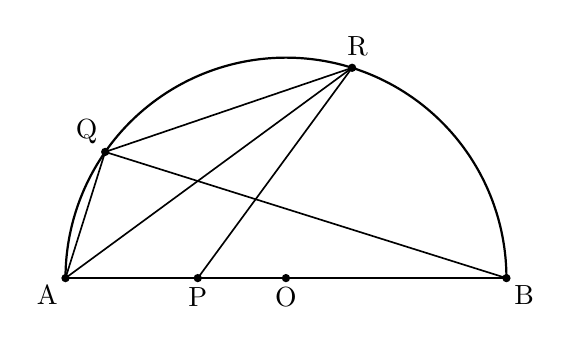
\begin{tikzpicture}

    % パラメータの定義
    \pgfmathsetmacro{\xmax}{5.6}
    \pgfmathsetmacro{\r}{\xmax/2}

    \pgfmathsetmacro{\rP}{2*\r/5}

    \pgfmathsetmacro{\thetaQ}{acos(((\r-\rP)^2 - 2*\r^2) / (2*\r^2))}

    % 点の定義
    \coordinate (O) at (0,0);
    \coordinate (A) at (180:\r);
    \coordinate (B) at (0:\r);

    \coordinate (P) at (180:\rP);
    
    \coordinate (Q) at (\thetaQ :\r);
    \coordinate (R) at (\thetaQ/2:\r);
    
    % 点の描画
    \fill (O) circle (1.5pt) node[below] {$\mathrm{O}$};
    \fill (A) circle (1.5pt) node[below left, outer sep=-.5pt] {$\mathrm{A}$};
    \fill (B) circle (1.5pt) node[below right, outer sep=-.5pt] {$\mathrm{B}$};
    \fill (P) circle (1.5pt) node[below] {$\mathrm{P}$};
    \fill (Q) circle (1.5pt) node[above left, outer sep=-.5pt] {$\mathrm{Q}$};
    \fill (R) circle (1.5pt) node[above, shift={(2pt,.8pt)}] {$\mathrm{R}$};

    % 半円の描画
    \draw [thick, domain=0:180, samples=250] plot ({\r*cos(\x)}, {\r*sin(\x)});

    % 線分の描画        
    \draw [thick] (A) -- (B);
    \draw [semithick] (A) -- (Q);
    \draw [semithick] (B) -- (Q);
    \draw [semithick] (A) -- (R);
    \draw [semithick] (P) -- (R);
    \draw [semithick] (R) -- (Q);

\end{tikzpicture}
\end{document}
 
